\documentclass{article}
\usepackage{preamble}

\title{ENGR3426: Miniproject 2}
\author{Jacob Smilg}
\date{September 26th 2023}

\urlstyle{same}
\begin{document}

\maketitle

\section{Schematic Capture and Simulation}

\begin{figure}[!ht]
    \centering
    \includesvg[inkscapelatex=false, width=.9\columnwidth]{../shiftreg_tran_harness.svg}
    \caption{Schematic of my four-bit shift register simulation test harness created in Xschem.}\label{fig:sim_schem}
\end{figure}

\begin{figure}[!ht]
    \centering
    \includesvg[inkscapelatex=false, width=.6\columnwidth]{../flipflop_layout.svg}
    \caption{Layout-driven schematic of my D flip-flop created in Xschem. The dimensions of M5 and M10 are altered to account for the non-ratio-less-ness of the CSRL design.}\label{fig:flipflop_schem}
\end{figure}

\begin{figure}[!ht]
    \centering
    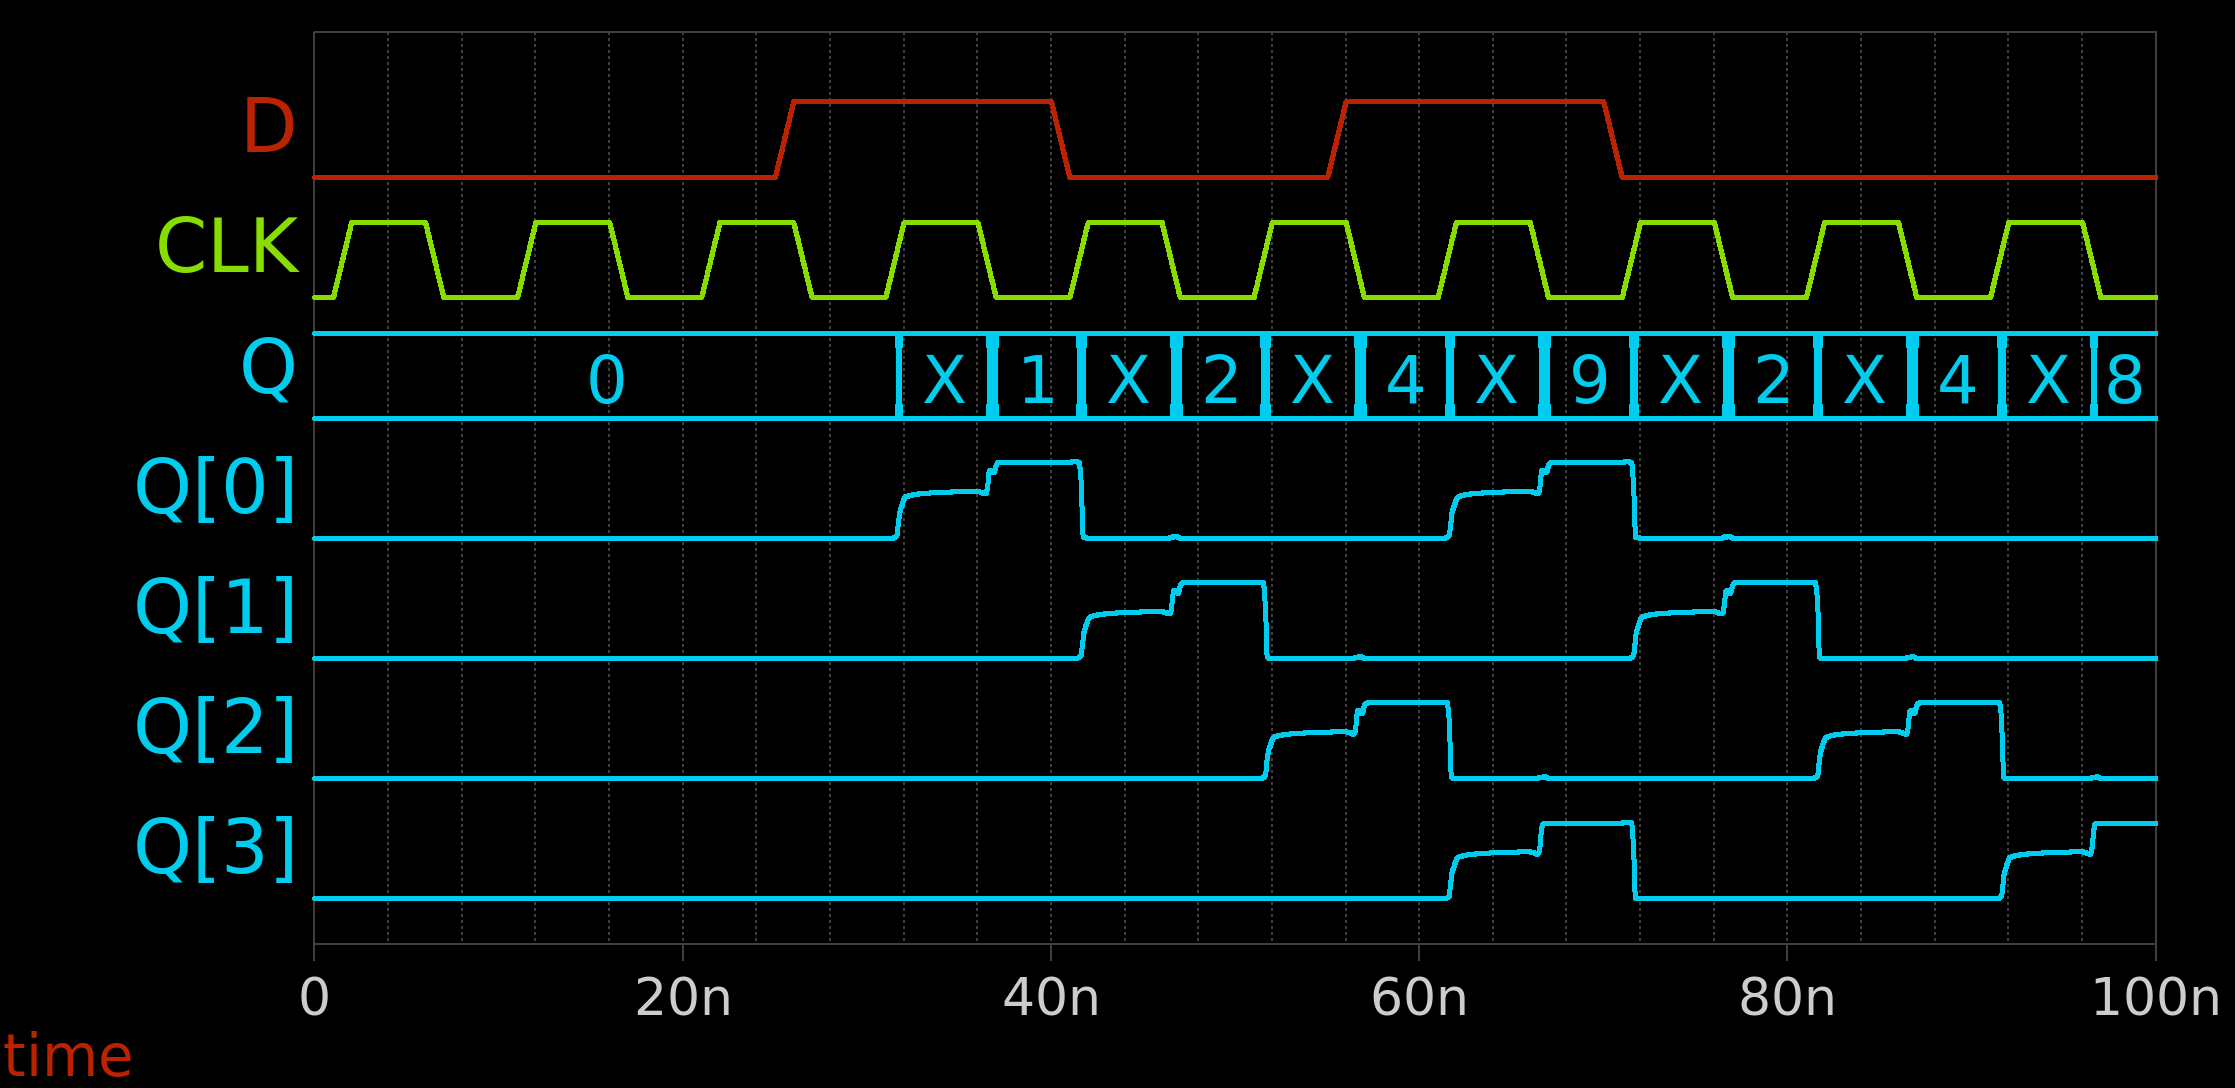
\includegraphics[width=.9\columnwidth]{../simulation/stackedplot.png}
    \caption{A plot of the output of the simulation of Figure~\ref{fig:sim_schem}. The shift register behaves as expected; the state of D propagates through the flip-flops on each rising edge of CLK.}\label{fig:simplot}
\end{figure}

\clearpage

\section{Layout Design}

\begin{figure}[!ht]
    \centering
    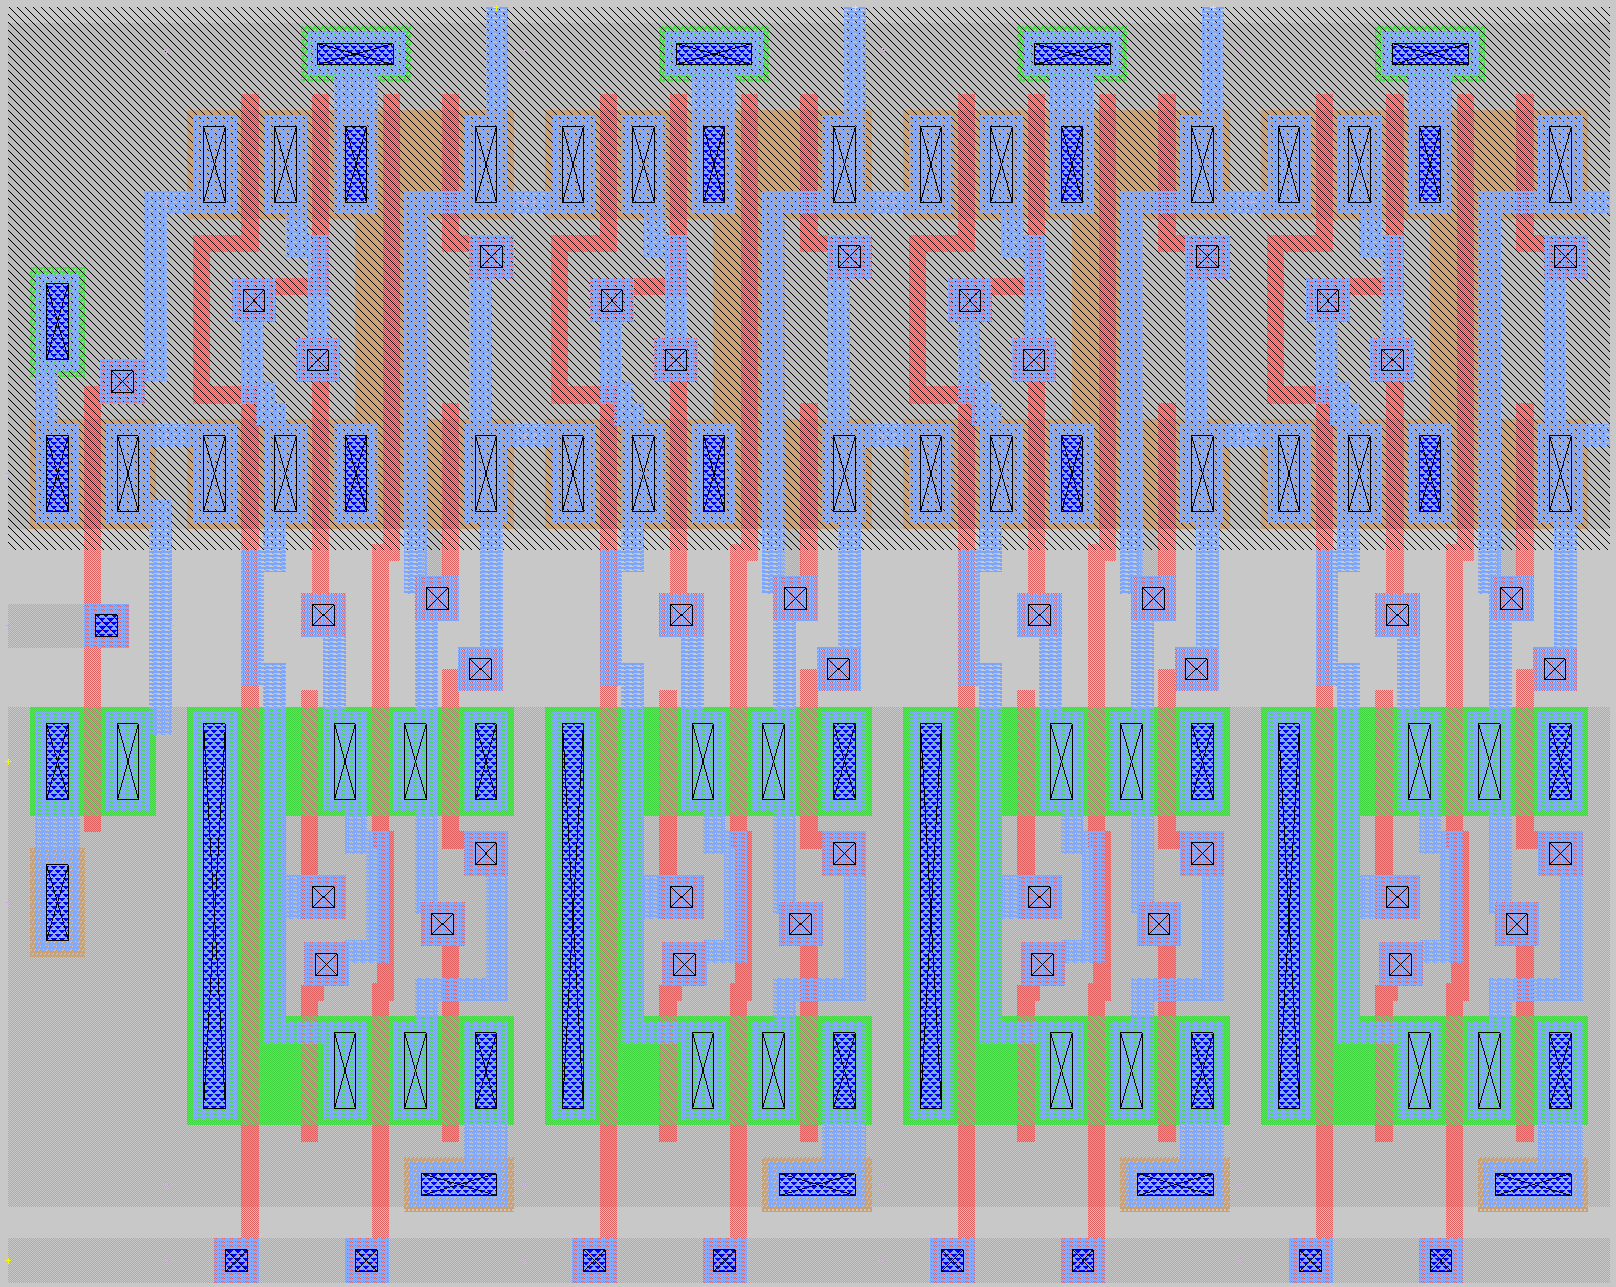
\includegraphics[width=\columnwidth]{../layout/shiftreg.png}
    \caption{A screenshot of the top-level layout of my four-bit shift register. The overall width of the shift register is 14.750 microns, and the height is 11.750 microns.}\label{fig:layout_top}
\end{figure}

\begin{figure}[!ht]
    \centering
    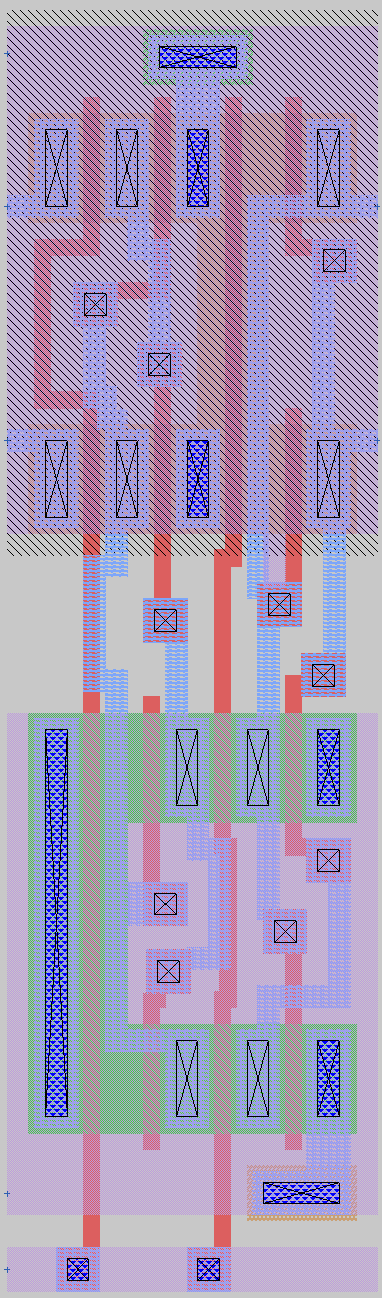
\includegraphics[width=.375\columnwidth]{../layout/flipflop.png}
    \caption{A screenshot of the cell layout of my D flip-flop. The clock signal and power and ground rails are routed horizontally in a metal layer, and the input enters the cell on the left and propagates to the right.}\label{fig:layout_flipflop}
\end{figure}

\clearpage

\section{Layout Versus Schematic}

\begin{figure}[h]
    \centering
    \includesvg[inkscapelatex=false, width=.9\columnwidth]{../shiftreg.svg}
    \caption{Schematic of my shift register separated from the simulation test harness for LVS.}\label{fig:lvs_schem}
\end{figure}

\subsection{LVS Output Log}

The following is the contents of the file \texttt{mp2/comp.out} obtained from running the netgen LVS program comparing \texttt{mp2/layout/shiftreg.spice} (Magic netlist) and \texttt{mp2/simulation/shiftreg.spice} (Xschem netlist). It shows that the layout and schematic match.

\lstset{%
    breaklines=true,
    breakatwhitespace=true,
}
\lstinputlisting{../comp.out}

\section{Design Files}

All of the files for this miniproject can be found at \url{https://github.com/smilg/madvlsi-fa23/tree/main/mp2}.

\end{document}